\chapter[Resultados obtidos]{Resultados Obtidos}

O desenvolvimento do Traveller foi, desde seu início, fortemente testado por uma suíte de testes que garantiam a integridade do código em um ambiente de mudanças constantes. Assim, foi possível garantir que mesmo inserindo novos códigos, módulos e alterando as classes já existentes, as funções continuavam em funcionamento. Quando alguma alteração mudava os resultados das saídas, os testes acusavam imediatamente.

Porém, para uma suíte de testes garantir essa integridade, os testes realizados precisam cobrir as áreas passíveis de falhas e críticas do sistema. Um teste que verifica uma função muito simples ou que nunca muda não nos confere tanta integridade do sistema como uma que verifica se o sistema responde corretamente ao entrar com um mapa, o qual não permite chegar ao destino final. Para isso, a suíte de testes foi constantemente avaliada e revisada, buscando uma maior qualidade dos testes realizados.

A seguir serão descritos os testes realizados durante o desenvolvimento do Traveller \textit{Framework} e os impactos dos mesmos no desenvolvimento do sistema.

\section{Testes iniciais}

Ao iniciar o desenvolvimento do \textit{framework}, foram desenhados sete mapas simples apenas para testar se os algoritmos estavam funcionando. Os mapas desenhados eram pequenos, permitindo calcular o grafo gerado e o menor caminho manualmente. Os mapas variavam  de 4 a 9 células de largura, podendo ser quadradas ou retangulares. A mudança de tamanho e formato permitiu testar as divisões em áreas do Quadtree e verificar se o mesmo repartia como planejado. Para esses exemplos iniciais não foi considerados: (i) a expansão dos obstáculos, e (ii) que o robô e a célula possuíam o mesmo tamanho. A saídas de cada classe (o grafo e a lista de pontos) foram testadas para cada caso. A classe \textit{controller} não foi usada, permitindo acesso ao grafo e a verificação e validação do mesmo. A figura 35 mostra um destes testes.

\begin{figure}[h]
	\centering
	\label{fig35}
		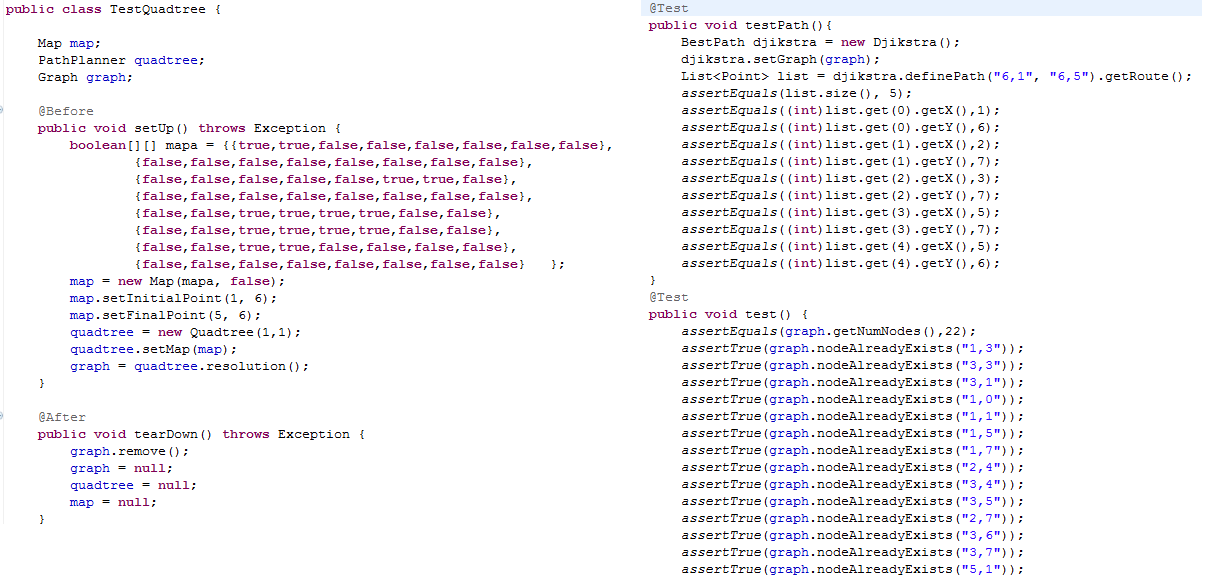
\includegraphics[keepaspectratio=true,scale=0.6]{figuras/testeinicial.png}
	\caption{Teste inicial do \textit{framework}}
\end{figure}

\section{Testes de desempenho}

Após a validação do tema e verificado o funcionamento correto do fluxo de trabalho do \textit{framework}, o próximo passo foi o teste de desempenho do mesmo. Foram analizados o consumo de memória e o tempo de processamento para a avaliação do mesmo. 

Os testes foram realizados na IDE Netbeans, usando sua ferramenta de perfis. Esta ferramenta permite avaliar a memória que a JVM (\textit{Java Virtual Machine}) está consumindo e o tempo de processamento de um programa, tomando como base cada método e classe. Ela fornece o número de vezes que um método é chamado, o tempo total para execução dos mesmos, o tempo requerido para execução de toda a classe e a porcentagem de cada um.

O algoritmo utilizado nestes testes foi o Quadtree. Este algoritmo permitiu uma análise mais rigorosa devido a sua implementação exigir maior memória para sua execução, através de sua recursão e de aumentar muito o número de objetos de acordo com o número e disposição dos obstáculos. Assim, foi analisado o \textit{framework} em seu pior caso, com mapas grandes, muitos obstáculos e com um algoritmo que cresce seu consumo junto com estas variantes.

\subsection{Testes de Stress - Simulação}

Os primeiros testes foram para testar os limites de processamento do Lego NXT, inserindo um mapa de 100 por 100 células e com uma enorme quantidade de obstáculos. Foram inseridos 1089 obstáculos (um a cada três casas) de 2 por 2 células. Dificilmente um ambiente assim seria utilizado para uso real. Entretanto, esse teste visava apenas avaliar o quanto o \textit{hardware} do robô utilizado suportava. As imagens 36 e 37 mostram o resultado da análise de processamento deste teste.

\begin{figure}[h]
	\centering
	\label{fig36}
		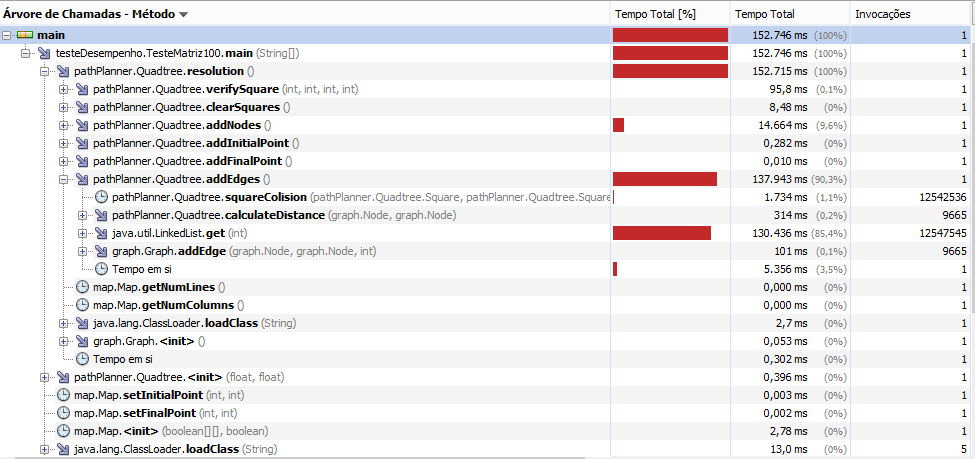
\includegraphics[keepaspectratio=true,scale=0.6]{figuras/teste100_1.PNG}
	\caption{teste de stress, tempo de execução}
\end{figure}

\begin{figure}[h]
	\centering
	\label{fig37}
		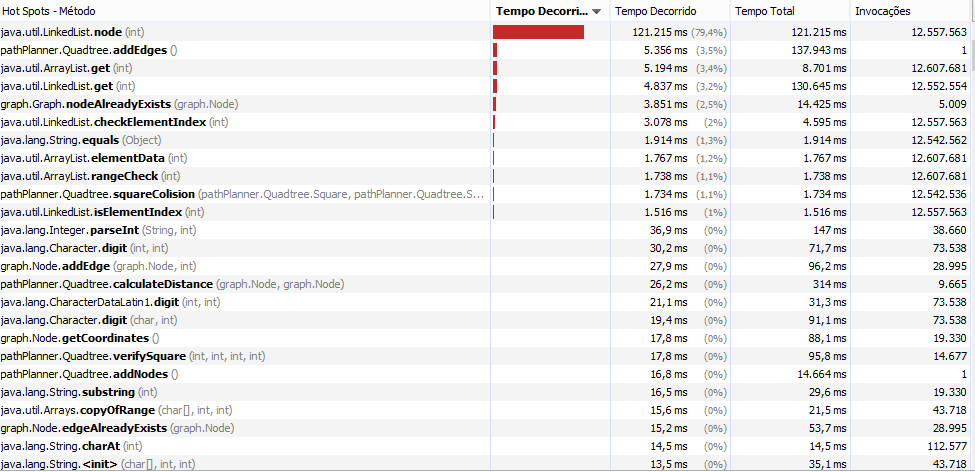
\includegraphics[keepaspectratio=true,scale=0.6]{figuras/teste100_2.PNG}
	\caption{teste de stress, métodos que mais foram utilizados}
\end{figure}

O teste levou ao todo quase 4 minutos para ser executado no computador, sendo este tempo repartido entre todos os processos da máquina e entre os vários processos dentro da própria máquina virtual Java. A análise retornou que o tempo gasto pelo \textit{framework} foi pouco mais de 152 milissegundos. A quantidade de tempo massiva gasta foi no método \textit{addEdges} do Quadtree (90,3\%), aonde 85,4\% do tempo total foi com o método \textit{get} do LinkedList e apenas 3,5\% do tempo foi com o método em si.

A figura 37 nos mostra que, neste mesmo teste, a classe LinkedList consumiu muito mais tempo de processador que as classes do próprio \textit{framework}. No total, a classe foi responsável por 85,5\% do tempo de processamento.

Com relação ao gasto de memória, a função que mais consumiu foi a classe Square, do Quadtree. Justamente pela imensa quantidade de obstáculos e o pouco espaço entre eles, o algoritmo gerou uma imensa quantidade de quadrados para a geração do grafo, consumindo boa parte da memória. Não foi possível determinar a quantidade exata de memória gasta, pois a ferramenta inidicava o gasto total da máquina virtual Java e não apenas o do processo estudado.

Um segundo teste foi realizado com o mesmo ambiente e os resultados foram os mesmos, com poucas mudanças em relação ao tempo.

\subsection{Testes de Stress no Robô}

Ao embarcar este código no robô, foi identificado um erro, devido à falta de memória. O tamanho do mapa foi diminuído para 30 por 30, mantendo a mesma proporção de obstáculos e o espaçamento entre eles. Mesmo com esta diminuição, ainda faltou memória no robô, precisando diminuir para 20 o tamanho do mapa. Foi medido com cronômetro digital que o tempo levado pelo \textit{framework} para calcular a trajetória com o mapa de 20x20 no robô foi de 15 segundos. Este mapa gerou um grafo com 500 nós e 1889 arestas. Este valor sozinho não pode definir o tamanho máximo de um grafo que o robô suporta (em um teste futuro, um mapa com grafo menor não executou), pois o tamanho do mapa e outras estrutras também ocupam a memória e afetam o limite da máquina.

Apesar de dificilmente haver um ambiente onde haja tantos obstáculos ou que o robô só possa se mover sobre uma grade, foi visto que mesmo com mapas pequenos a memória do Lego NXT não suporta o \textit{framework}. 

Outro teste feito no robô confirmou que o robô não suportaria o \textit{framework} para a maioria dos mapas. Nele, um mapa de 60x60 foi criado e inseridos apenas três obstáculos. Este mapa foi retirado do simulador MRIT, que trabalha com um mapa de 60x60 e três obstáculos inicialmente. 

Ao embarcá-lo no Lego, houve novamente estouro de memória. No grafo gerado por este mapa haviam 208 nós e 1060 arestas. O robô só conseguiu rodar o sistema ao retirar um dos obstáculos, gerando um grafo de 133 nós e 666 arestas. O tamanho do mapa foi mantido 60x60.

\subsection{Decisões tomadas}

Considerando que mesmo com mapas pequenos de 30x30 o Traveller pode não funcionar em alguns robôs e, principalmente, pelo teste com o mapa retirado do MRIT de 60x60 e 3 obstáculos não ter rodado no Lego, foi verificado que o consumo de memória do algoritmo Quadtree é muito alto e o \textit{framework} precisaria ser movido para fora do robô. Outros algoritmos, como o Wavefront e Grafo de Visibilidade, podem consumir bem menos memória, porém o \textit{framework} deve funcionar mesmo no pior caso. Dessa forma, a decisão de colocá-lo em um servidor foi tomada.

Vale lembrar que um mapa de 60x60 pode ainda ser pequeno dependendo da área de atuação do robô e do seu tamanho, já que a proporção entre robô e a área influencia no tamanho da matriz que o mesmo gerará.

Outra decisão foi a troca pela estrutura LinkedList pelo ArrayList. A grande maioria do tempo era gasto nesta classe, portanto, ela foi substituída por outra semelhante, também fornecida pelo Java. O ArrayList acessa um elemento com o método \textit{get} com ordem de complexidade O(1), enquanto o LinkedList faz o mesmo em ordem O(n). Mesmo o LinkedList apresentando vantagens quanto a gasto de memória e inserção e remoção de dados, essas funções eram pouco expressivas na totalidade do código, nem sequer chegando a aparecer nas estastísticas geradas. Enquanto a função \textit{get} estava sempre entre as que mais consumiam tempo.

\section{Testes unitários e de Integração}

Para a realização dos testes foi utilizada a ferramenta JUnit, que fornece classes para a realização de testes unitários. Estas classes foram aproveitadas para realizar outros tipos de testes, como os testes de integração explicados na seção 6.3.2.

A cada módulo construído e cada algoritmo implementado, uma nova suíte de testes era desenvolvida para validá-la. Outros detalhes sobre suas implementações são descritos nas seções a seguir.

\subsection{Testes unitários e cobertura de código}

Os testes unitários realizados buscavam a validação dos algoritmos, dos componentes e suas comunicações. Para tanto, foram realizado testes que chamavam as classes dos \textit{hot-spots} separadamente (sem se utilizar da controladora) para testar a saída de cada algoritmo.

Para os testes foram usados os mesmos mapas utilizados nos testes iniciais, que por seu tamanho reduzido permitiam calcular seus resultados manualmente para os quatro algoritmos e verificá-los com as funções do JUnit. Caso o algoritmo funcionasse nos casos testados, era considerado correto.

Para o diagrama de Voronoi houve uma maior dificuldade de implementar os testes unitários, mesmo em mapas menores e com menos obstáculos, devido a complexidade de seu algoritmo. Como o algoritmo fazia uso de diversos métodos privados, a maior parte do algoritmo não pôde ser testada diretamente pelos testes automátizados. Entretanto, testes manuais mostraram o correto funcionamento da maioria das funções internas, e que a falha estava presente na criação das triangulações de Delauney, o ponto central do algoritmo.

Como a maioria dos métodos que executam a lógica é privado, foi verificado diretamente pelas funções do JUnit apenas as saídas dos algoritmos e se as mesmas eram totalmente compatíveis com os valores esperados. Caso as saídas fossem compatíveis em todos os casos, então os métodos internos estariam corretos.

Algumas funções da classe \textit{Map} de maior complexidade e relevância também foram diretamente testadas. Os métodos de expansão dos obstáculos e de localizar e retornar os vértices dos obstáculos também foram verificados pela suíte de testes pela sua importância nos algoritmos por possuírem uma lógica mais elaborada que as demais da mesma classe. Quanto à expansão, foi expandido um obstáculo aonde o robô possuía o mesmo tamanho da célula da matriz (expanção de 1 célula), aonde o robô era menor (expansão também de 1 célula po arredondar para cima) e aonde o robô era 1,5 vezes maior (expansão de duas casas). Para a localização de vértices foram testados obstáculos retangulares, triangulares e hexagonais. Considerando que o mapa é uma matriz, todo polígono pentagonal ou maior à vizinhança do ponto seria a mesma.

Além do JUnit, foi utilizado também o plugin Eclemma para a cobertuda de código (Figura 38). Este plugin é executado juntamente com os testes unitários e marca as linhas executadas e qual a porcentagem do código foi verificada naquele teste. Como a execução do algoritmo executava todos os métodos internos, as classes eram testadas e cobertas em sua maioria. Ao final de todos os testes, foi alcançada uma cobertura de código de 94,4\%.

\begin{figure}[h]
	\centering
	\label{fig38}
		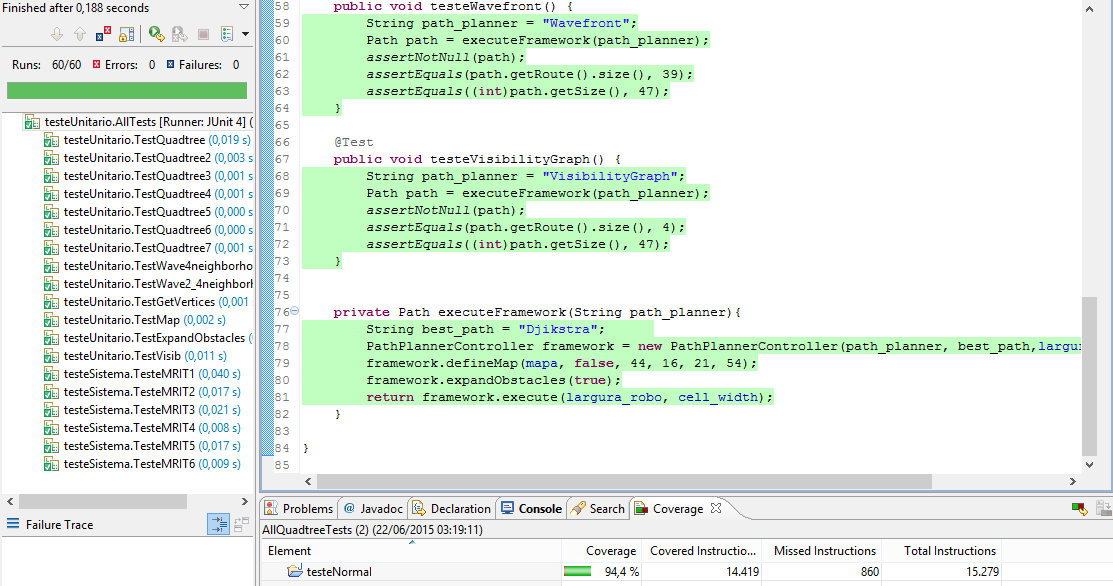
\includegraphics[keepaspectratio=true,scale=0.6]{figuras/cobertura.PNG}
	\caption{Cobertura de código do \textit{framework}}
\end{figure}

\subsection{Testes de Integração: Comparações Com o Simulador MRIT}

Além dos testes unitários, testando os métodos e os algoritmos de forma direta e atômica, foram realizados testes de integração, que testaram a comunicação entre os módulos do sistema. Esse grupo de testes é importante, pois após garantir que cada módulo funciona de forma correta, é preciso garantir que eles se comunicam de forma correta também.

Para tanto, foram montado seis cenários a serem testados. Para a comparação dos algoritmos e validação de seu funcionamento com o simulador MRIT, foram criados seis mapas no simulador e definida suas trajetórias para cada algoritmo. Estes mapas foram também criados no \textit{framework}, com o mesmo tamanho e os obstáculos nas mesmas posições para a comparação dos resultados.

Uma vez montado os seis mapas, foi definido o algoritmo de menor caminho como Djikstra e executado o \textit{framework} para cada um dos algoritmos de definição de trajetória. A execução foi feita a partir da controladora PathPlannerController, do mesmo modo que o módulo \textit{Main} o executa. Assim, foi testado o módulo controlador e sua integração com os módulos PathPlanner, Map e BestPath. Todo o fluxo de trabalho foi executado em cada teste, criando o mapa, instanciando os algoritmos, expandido os obstáculos caso fosse definido pelo teste e, por fim, executado ambos os algoritmos, gerando o grafo, passando-o para o BestPath e gerando a lista de pontos no final. Com estas verificações, foi possível validar que o Traveller funcionava como um todo e que respondia corretamente as entradas dos dados e gerava a saída de forma correta.

As figuras 39 à 44 mostram os mapas montados no simulador MRIT. As trajetórias em vermelho foram geradas pelo simulador, enquanto as azuis foram geradas pelo Traveller. Uma observação importante a ser feita é que tanto o simulador MRIT quanto o Traveller podem não retornar uma trajetória caso não consigam encontrar um caminho. Para o mapa 3, o MRIT não conseguiu encontrar uma solução para o Wavefront, para o mapa 5 não encontrou um caminho para o Voronoi e para o mapa 6 o único algoritmo a encontrar um percurso foi o Grafo de Visibilidade. Uma curiosidade interessante é que, quando o simulador não consegue gerar um percurso, os obstáculos somem, ficando apenas os pontos inicial e final no mapa (como visível nas Figuras 41, 43 e 44).

Quanto ao Traveller, para os seis mapas criados, apenas o Voronoi apresentou problemas, sendo encontrado um resultado apenas para o primeiro mapa. No sexto mapa, além do Voronoi, o Quadtree também não encontrou um caminho. Isso se deve a ambos recortarem os ambientes livres em áreas e nenhum dos dois encontrar um espaço grande o suficiente para criar as áreas necessárias para ligar os pontos inicial e final.

\begin{figure}[h]
	\centering
	\label{fig39}
		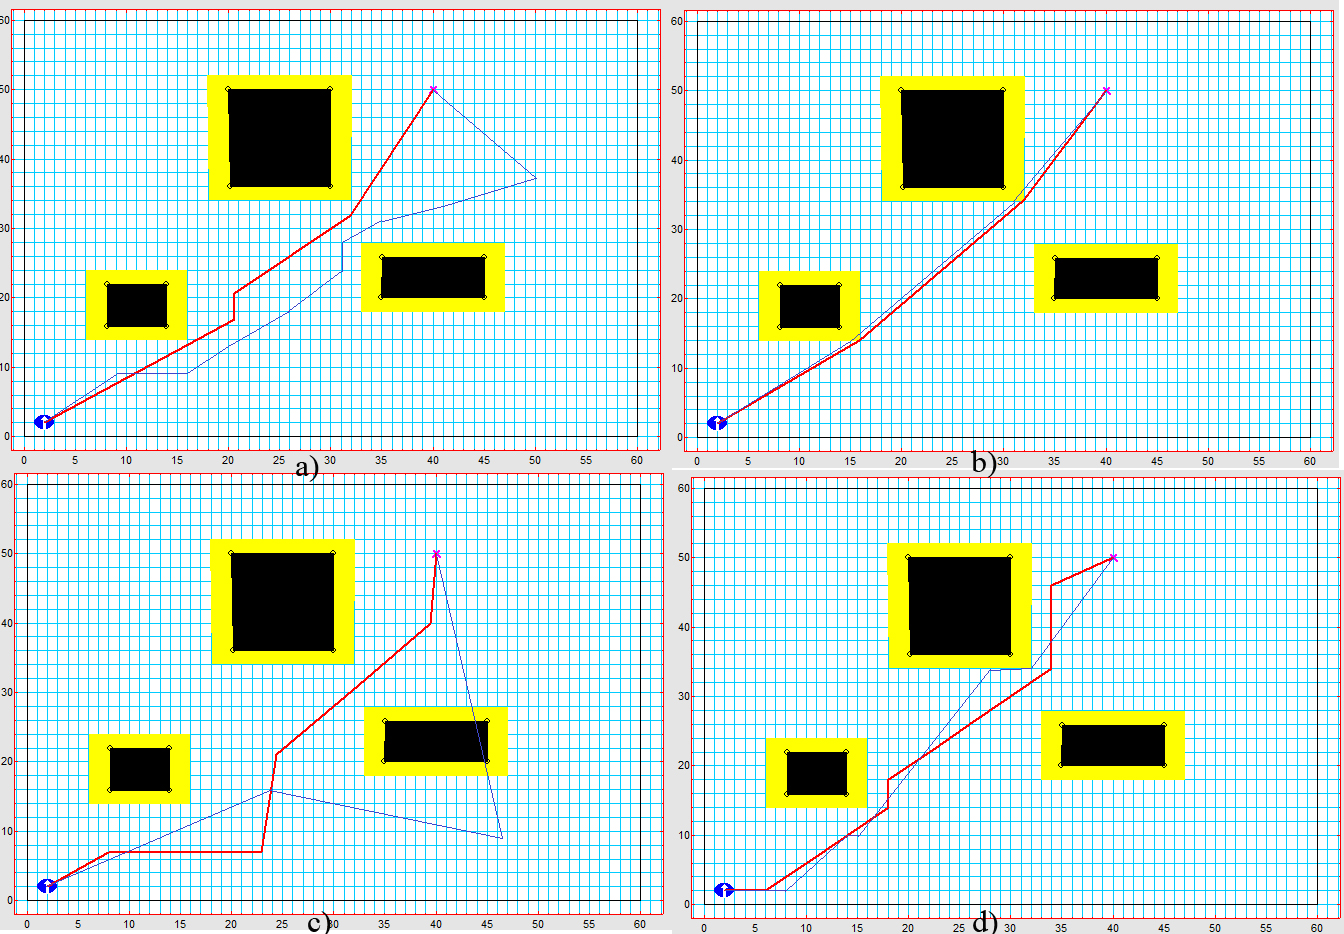
\includegraphics[keepaspectratio=true,scale=0.3]{figuras/mapa1.jpg}
	\caption{Trajetórias para o mapa 1 (MRIT em vermelho e Traveller em azul) a) Quadtree, b) Grafo de Visibilidade, c) Voronoi, d) Wavefront}
\end{figure}

\begin{figure}[H]
	\centering
	\label{fig40}
		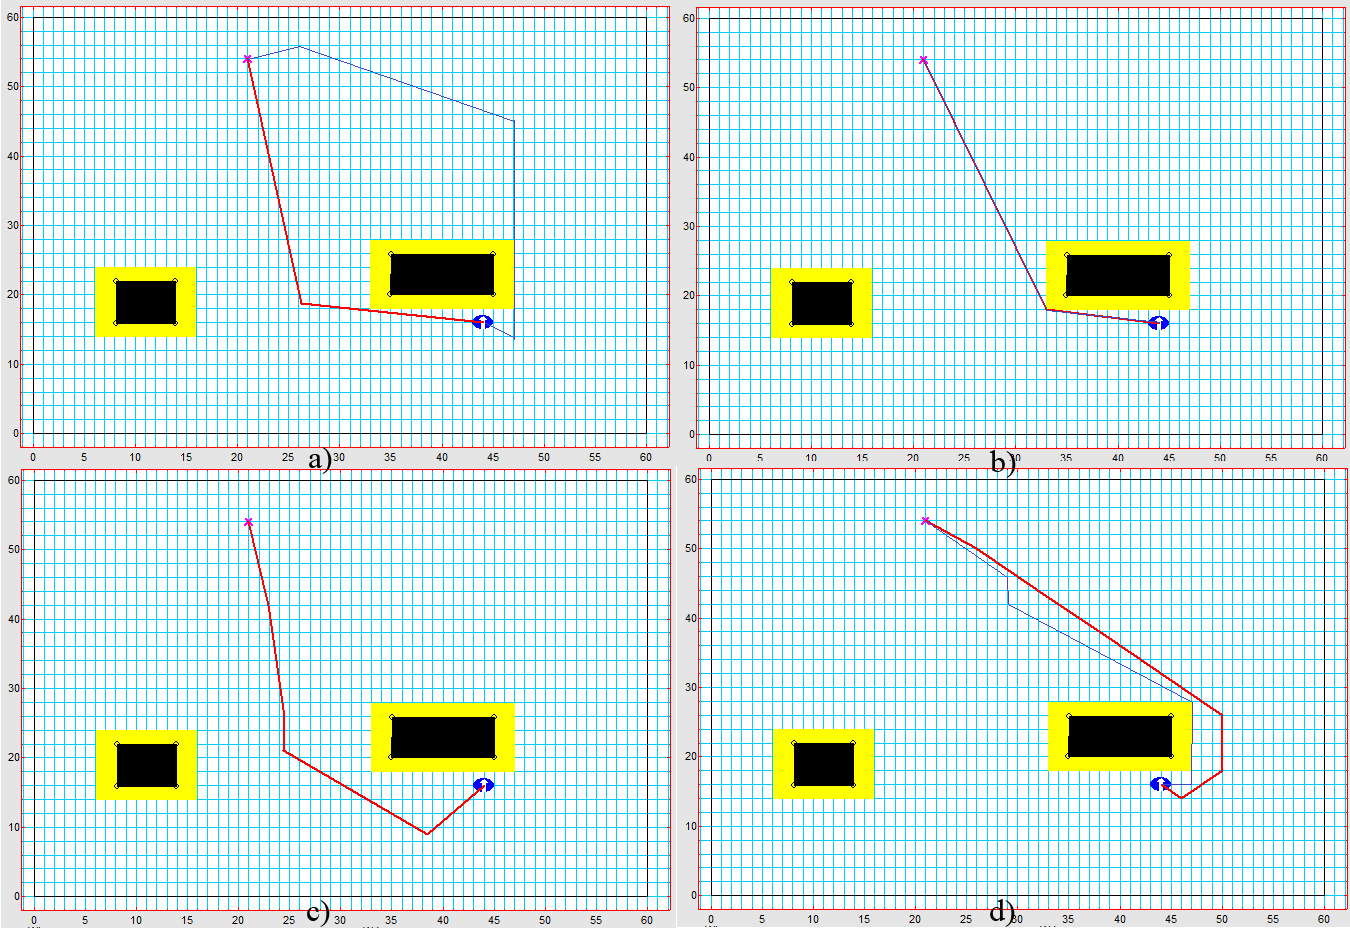
\includegraphics[keepaspectratio=true,scale=0.3]{figuras/mapa2.jpg}
	\caption{Trajetórias para o mapa 2 (MRIT em vermelho e Traveller em azul) a) Quadtree, b) Grafo de Visibilidade, c) Voronoi, d) Wavefront}
\end{figure}

\begin{figure}[H]
	\centering
	\label{fig41}
		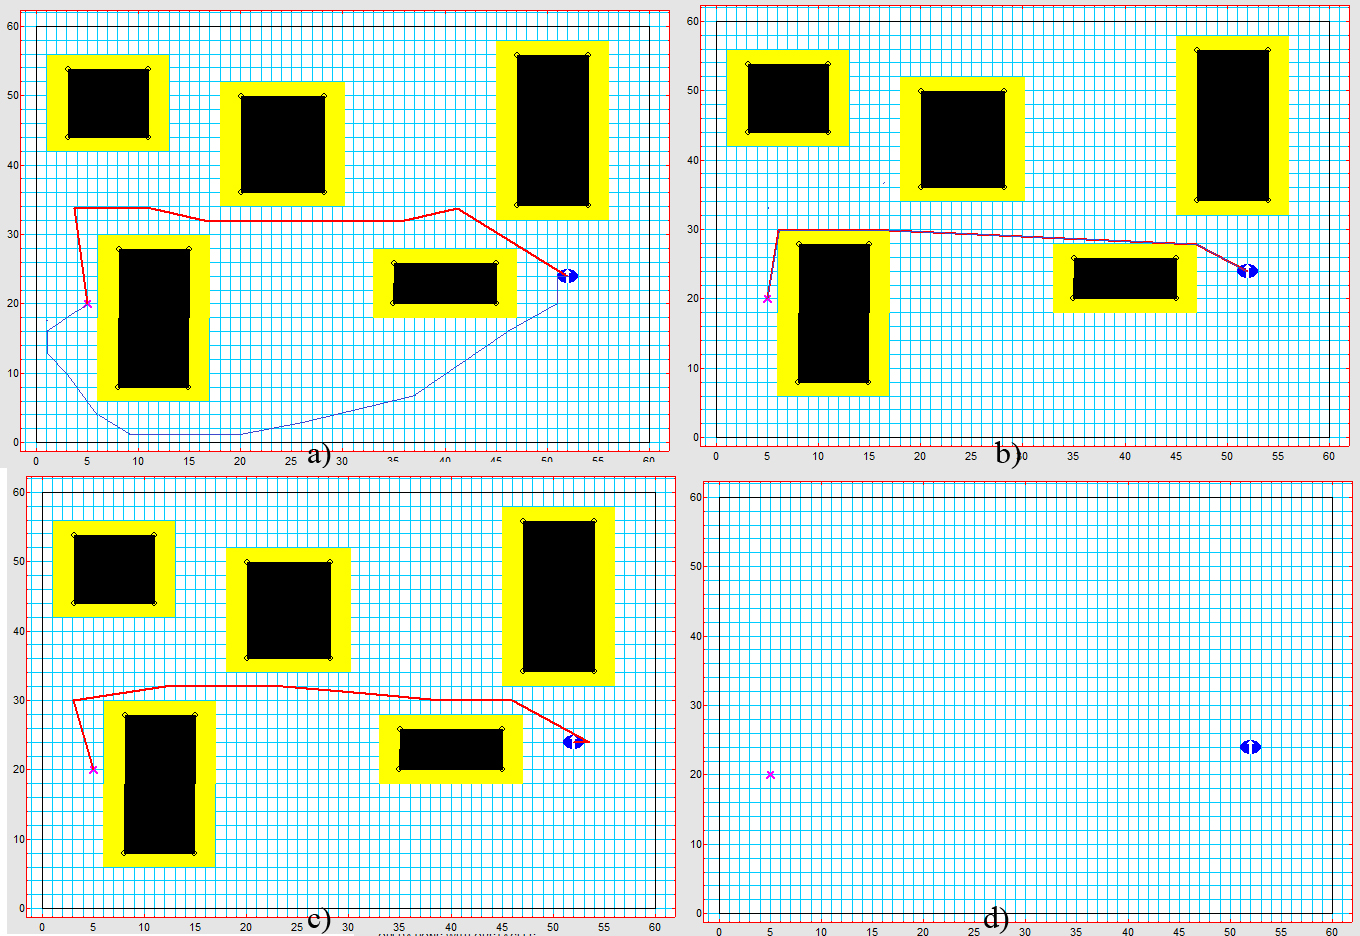
\includegraphics[keepaspectratio=true,scale=0.3]{figuras/mapa3.jpg}
	\caption{Trajetórias para o mapa 3 (MRIT em vermelho e Traveller em azul) a) Quadtree, b) Grafo de Visibilidade, c) Voronoi, d) Wavefront}
\end{figure}

\begin{figure}[H]
	\centering
	\label{fig42}
		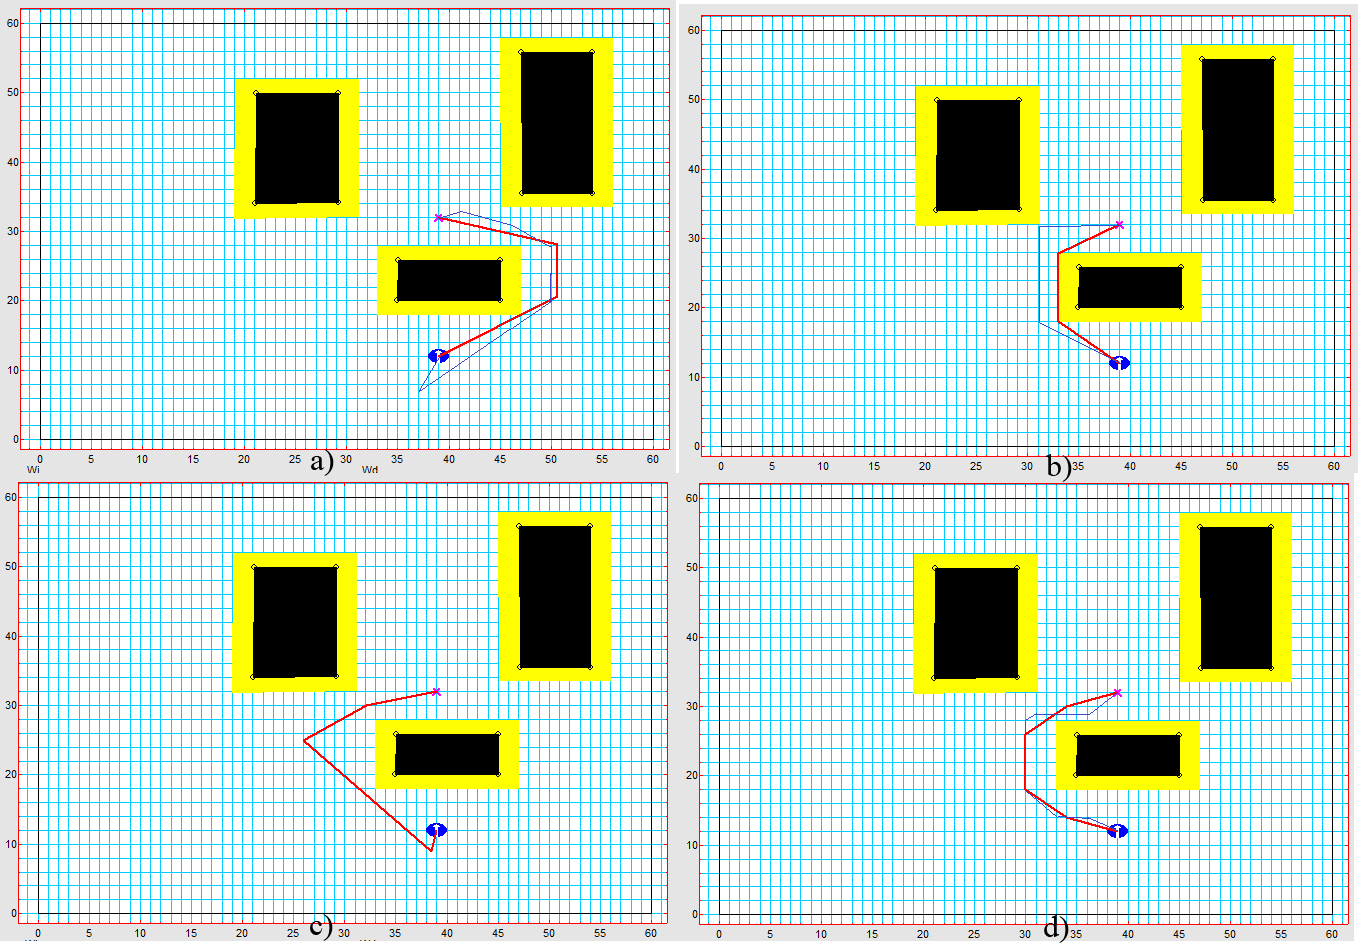
\includegraphics[keepaspectratio=true,scale=0.3]{figuras/mapa4.jpg}
	\caption{Trajetórias para o mapa 4 (MRIT em vermelho e Traveller em azul) a) Quadtree, b) Grafo de Visibilidade, c) Voronoi, d) Wavefront}
\end{figure}

\begin{figure}[H]
	\centering
	\label{fig43}
		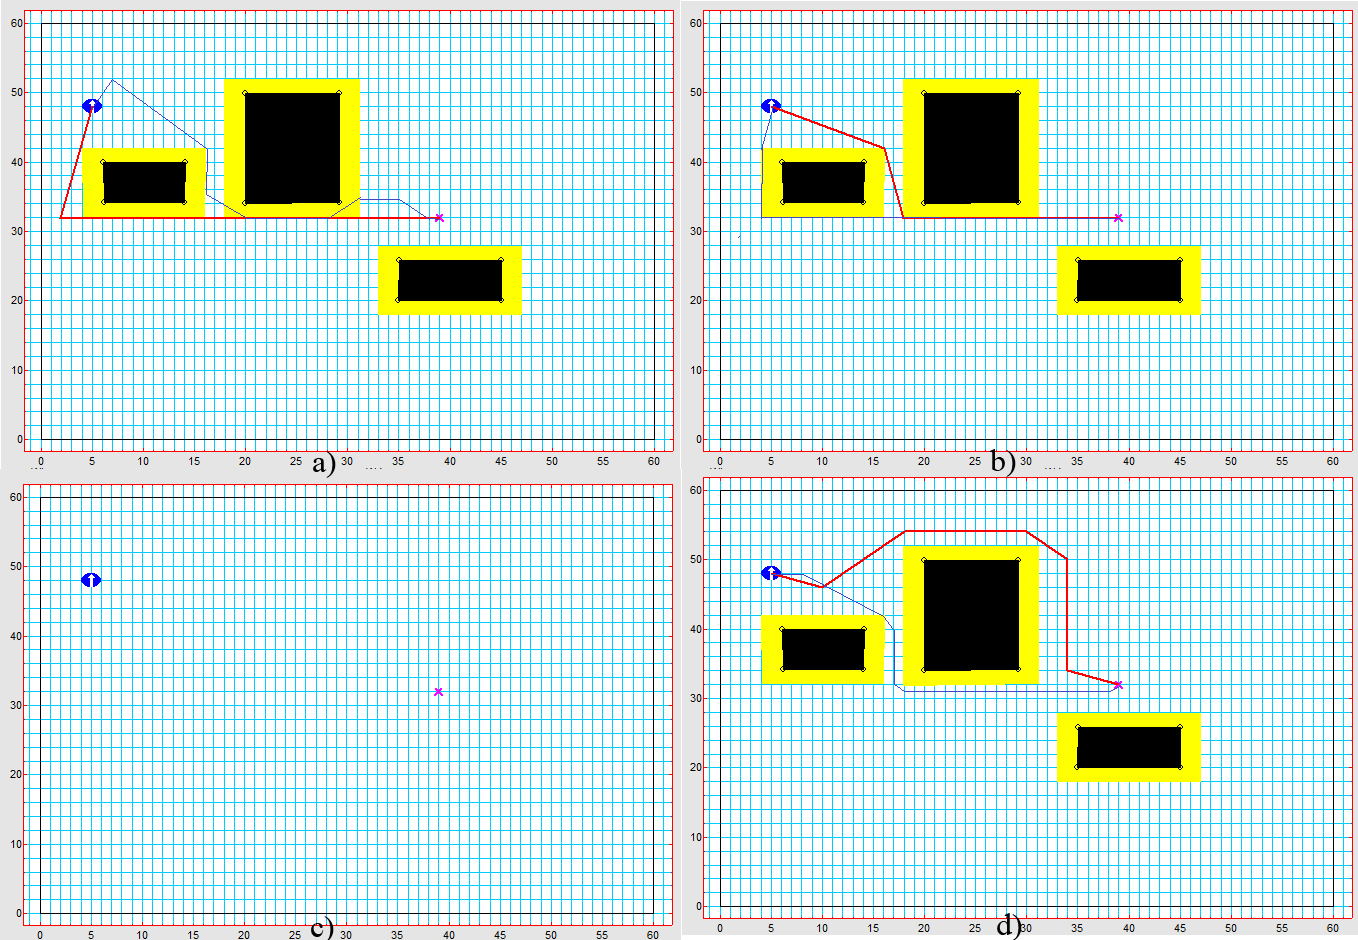
\includegraphics[keepaspectratio=true,scale=0.3]{figuras/mapa5.jpg}
	\caption{Trajetórias para o mapa 5 (MRIT em vermelho e Traveller em azul) a) Quadtree, b) Grafo de Visibilidade, c) Voronoi, d) Wavefront}
\end{figure}

\begin{figure}[H]
	\centering
	\label{fig44}
		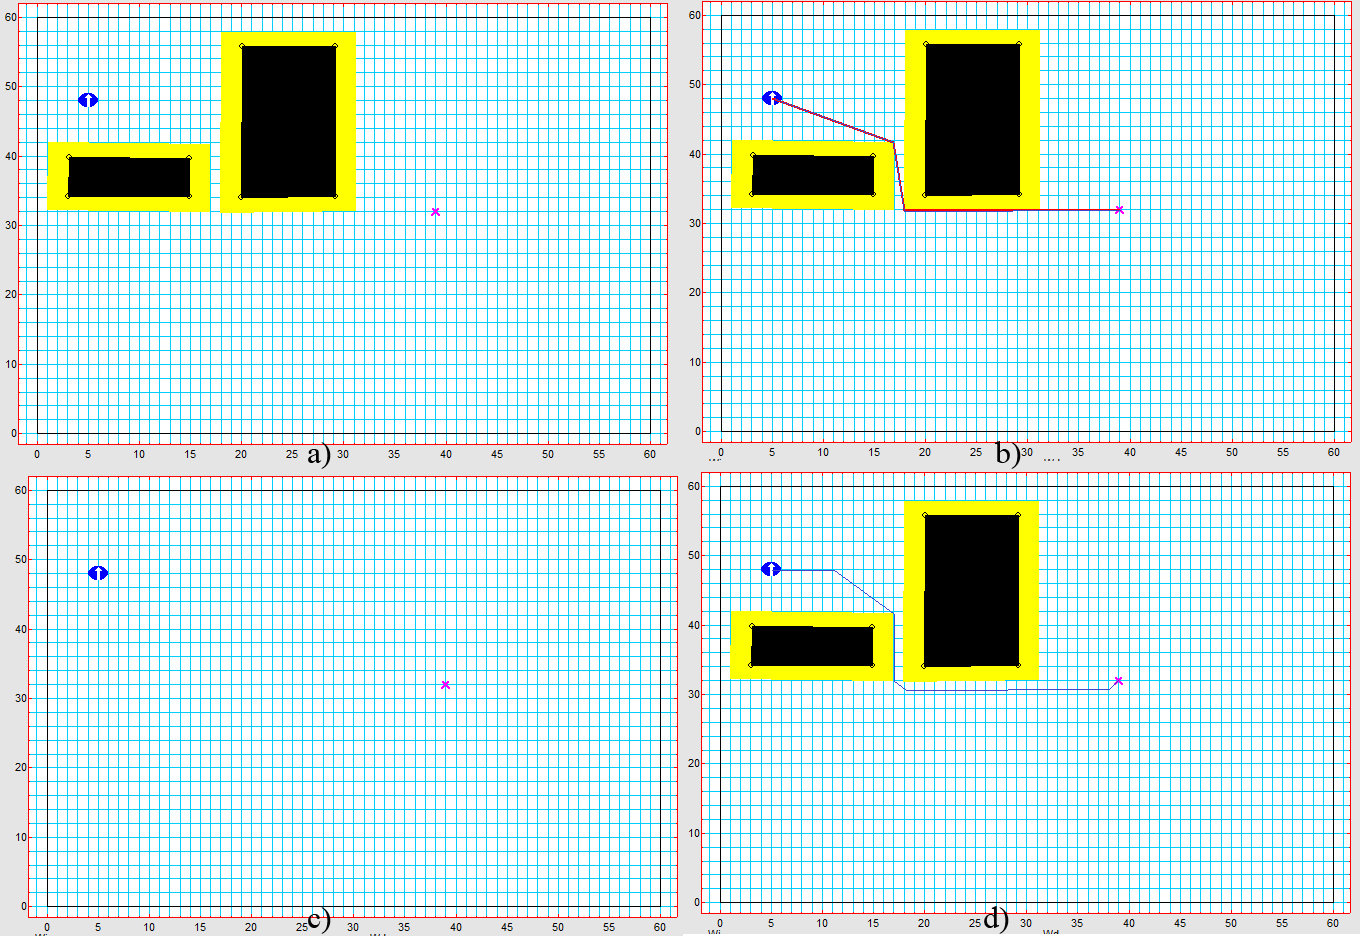
\includegraphics[keepaspectratio=true,scale=0.3]{figuras/mapa6.jpg}
	\caption{Trajetórias para o mapa 6 (MRIT em vermelho e Traveller em azul) a) Quadtree, b) Grafo de Visibilidade, c) Voronoi, d) Wavefront}
\end{figure}

Considerando as seis amostras, é possível analisar algumas semelhanças e diferenças entre as implementações dos algoritmos do simulador MRIT e do Traveller.

Nos resultados do \textit{framework}, o Quadtree nem sempre parece está se digirindo ao ponto final. Ele pode, em alguns casos, seguir para outras direções ao longo do percurso, para depois virar em direção ao objetivo. Esse comportamento fez com que o Quadtree gerasse um caminho maior, com exceção do mapa 5. Foi observado também que diversas vezes o algoritmo do \textit{framework} contornou o obstaculo por um lado diferente do simulador, o que indica que a divisão do mapa em retângulos foi implementada d eforma diferente do simulador. O percurso gerado pelo Traveller também gerou um caminho menos retilíneo.

Para o algoritmo Grafo de Visibilidade, o \textit{framework} gerou o mesmo caminho ou um muito proximo do simulador. Para o mapa 2 o caminho foi exatamnte o mesmo e, para os mapas 1 e 4, acredita-se que o caminho só não foi igual devido a um erro na implementação dos limites do mapa na suíte de testes. O Grafo de Visibilidade implementado pelo Traveller seguiu exatamente o que se esperava do algoritmo.

Como já comentado, o algoritmo Voronoi não conseguiu chegar a um resultado satisfatório. Para os seis mapas, apenas para o primeiro o algoritmo conseguiu gerar um caminho. Pelos testes realizados durante sua implementação, a falha no algoritmo está presente na criação dos triângulos de Delauney e validação das arestas destes triângulos.

Quanto ao algoritmo Wavefront, para os mapas 3 e 6 o simulador não conseguiu gerar um resultado, enquanto o \textit{framework} conseguiu. Quanto aos percursos gerados,
estes não mudaram tanto, seguindo mais ou menos a mesma trajetória. A única exceção foi o mapa 5, em que o percurso do \textit{framework} passou por baixo de um obstaculo, diminuindo o caminho, enquanto o simulador foi por cima. O \textit{framework} gerou um caminho significativamente menor para a maioria dos casos, obtendo um resultado pior apenas para o mapa 4, onde a diferença foi mínima (1,9 unidades).

O tamanho dos percursos gerados por cada algoritmo em cada mapa pode ser visto nas Tabela 1 à 6.

\begin{table}[h]
	\centering
	\label{tab01}
	\begin{tabular}{ccc}
		\toprule
		\textbf{Algoritmo} & \textbf{Traveller} & \textbf{MRIT} \\
		\midrule
Grafo de Visibilidade & 63.23   & 61.94 \\
Voronoi 				  & 80.84   & 60.79 \\
Quadtree				  & 68.81   & 63.78 \\
Wavefront             & 63.2    & 67.88  \\
		\bottomrule
	\end{tabular}
	\caption{Tamanho dos percursos gerados pelo simulador e o \textit{framework} para o mapa 1}
\end{table}

\begin{table}[H]
	\centering
	\label{tab02}
	\begin{tabular}{ccc}
		\toprule
		\textbf{Algoritmo} & \textbf{Traveller} & \textbf{MRIT} \\
		\midrule
Grafo de Visibilidade & 49.13   & 49.13 \\
Voronoi 				  & X       & 87 \\
Quadtree				  & 58      & 54.46 \\
Wavefront             & 50.2    & 56.8  \\
		\bottomrule
	\end{tabular}
	\caption{Tamanho dos percursos gerados pelo simulador e o \textit{framework} para o mapa 2}
\end{table}

\begin{table}[H]
	\centering
	\label{tab03}
	\begin{tabular}{ccc}
		\toprule
		\textbf{Algoritmo} & \textbf{Traveller} & \textbf{MRIT} \\
		\midrule
Grafo de Visibilidade & 57.57   & 57.52 \\
Voronoi 				  & X   		& 77.88 \\
Quadtree				  & 77.38   & 66.57 \\
Wavefront             & 54.6    & X  \\
		\bottomrule
	\end{tabular}
	\caption{Tamanho dos percursos gerados pelo simulador e o \textit{framework} para o mapa 3}
\end{table}

\begin{table}[H]
	\centering
	\label{tab04}
	\begin{tabular}{ccc}
		\toprule
		\textbf{Algoritmo} & \textbf{Traveller} & \textbf{MRIT} \\
		\midrule
Grafo de Visibilidade & 32   & 25.70 \\
Voronoi 				  & X   & 39.14 \\
Quadtree				  & 42   & 33.98 \\
Wavefront             & 32    & 30.1  \\
		\bottomrule
	\end{tabular}
	\caption{Tamanho dos percursos gerados pelo simulador e o \textit{framework} para o mapa 4}
\end{table}

\begin{table}[H]
	\centering
	\label{tab05}
	\begin{tabular}{ccc}
		\toprule
		\textbf{Algoritmo} & \textbf{Traveller} & \textbf{MRIT} \\
		\midrule
Grafo de Visibilidade & 40.9   & 43.73 \\
Voronoi 				  & X      & X \\
Quadtree				  & 53.1   & 53.28 \\
Wavefront             & 42.2    & 55.75  \\
		\bottomrule
	\end{tabular}
	\caption{Tamanho dos percursos gerados pelo simulador e o \textit{framework} para o mapa 5}
\end{table}

\begin{table}[H]
	\centering
	\label{tab06}
	\begin{tabular}{ccc}
		\toprule
		\textbf{Algoritmo} & \textbf{Traveller} & \textbf{MRIT} \\
		\midrule
Grafo de Visibilidade & 55.2   & 33.21 \\
Voronoi 				  & X      & X \\
Quadtree				  & X      & X \\
Wavefront             & 47.2    & X  \\
		\bottomrule
	\end{tabular}
	\caption{Tamanho dos percursos gerados pelo simulador e o \textit{framework} para o mapa 6}
\end{table}

\subsection{Testes de Integração: Desempenho}

Foi também verificado o desempenho do \textit{framework} diante da execução de todo seu fluxo de dados. O primeiro teste feito foi uma comparação entre os métodos LinkedList e ArrayList. Foi executado o mapa 1 com LinkedList em seus métodos e, após isso, substituído todos por ArrayList e executado o teste novamente. As diferenças de tempo podem ser vistas nas Figuras 45 e 46.

\begin{figure}[h]
	\centering
	\label{fig45}
		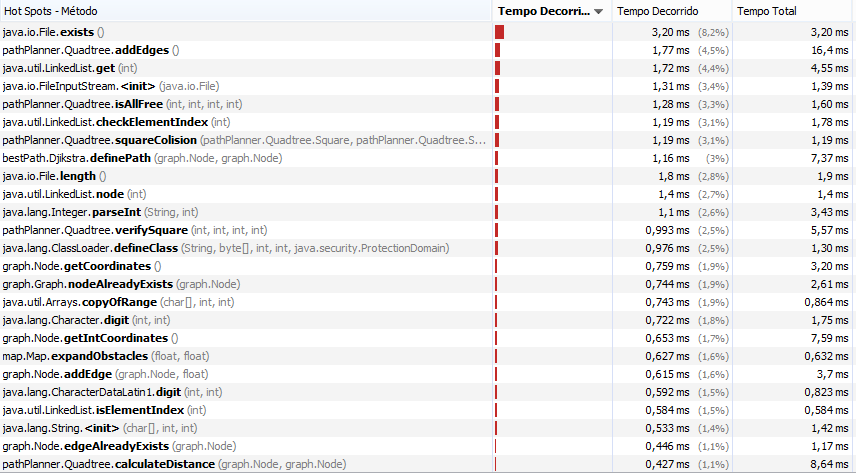
\includegraphics[keepaspectratio=true,scale=0.6]{figuras/link.PNG}
	\caption{tempo de processamento do mapa 1 com LinkedList}
\end{figure}

\begin{figure}[h]
	\centering
	\label{fig46}
		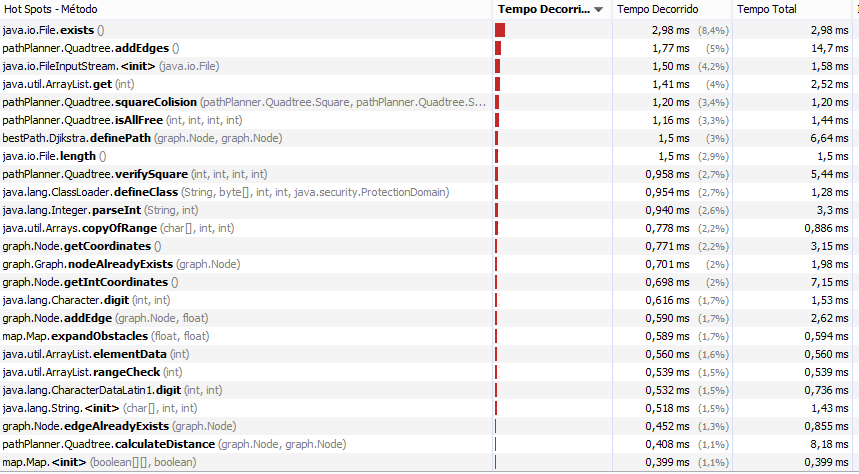
\includegraphics[keepaspectratio=true,scale=0.6]{figuras/array.PNG}
	\caption{tempo de processamento do mapa 1 com ArrayList}
\end{figure}

Com o LinkedList, o \textit{framework} levou 39,2 milisegundos para ser executado e a função get levou, ao total de todas as suas chamadas, 1,72 milisegundos de processamento. Ao substituir para ArrayList, o tempo total decaiu para 35,47 milisegundos e o tempo da função get caiu para 1,41 milisegundos. A diferença de 3,73 milisegundos foi o suficiente para levar a mudança de todas as estruturas para ArrayList.

Uma vez que todo o \textit{framework} usava ArrayList, foi testado o desempenho de todos os algoritmos nos seis mapas. Nas figuras 47 à 50 é mostrado o resultado do processamento para o mapa 3. Ao avaliar os 24 resultados, foi analisado o desempenho de cada algoritmo para as variados tipos de ambiente. O tempo médio das simulações foi de: 32.1 milisegundos para o Quadtree, 18.4 milisegundos para o Grafo de Visibilidade, 70 milisegundos para o Voronoi e 167 milisegundos para o Wavefront. Portanto, pela simulação, o Wavefront levou muito mais tempo para ser calculado que os demais algoritmos e o Voronoi consumiu um tempo considerável a mais que o Quadtree e o Grafo de Visibilidade. Também foi observado que, nas simulações, o Grafo de Visibilidade teve um desempenho mais uniforme, com pouca variação entre seus tempos.

Em todos os casos, o tempo do algoritmo de definição de trajetória foi muito maior que o de definição de menor caminho e, de todo o fluxo, a definição de trajetória e os métodos de outras classes chamadas dentro dele ocuparam sempre mais de 50\% do processador.

\begin{figure}[h]
	\centering
	\label{fig47}
		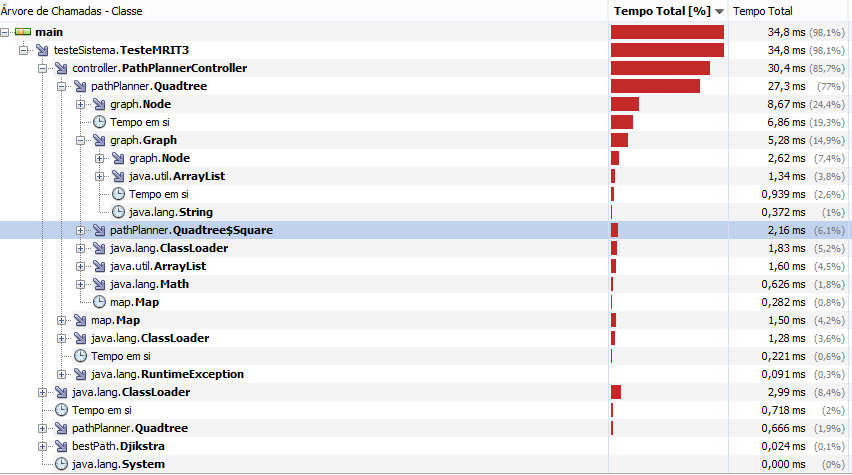
\includegraphics[keepaspectratio=true,scale=0.6]{figuras/quad3.PNG}
	\caption{tempo de processamento do mapa 3 com Quadtree}
\end{figure}

\begin{figure}[H]
	\centering
	\label{fig48}
		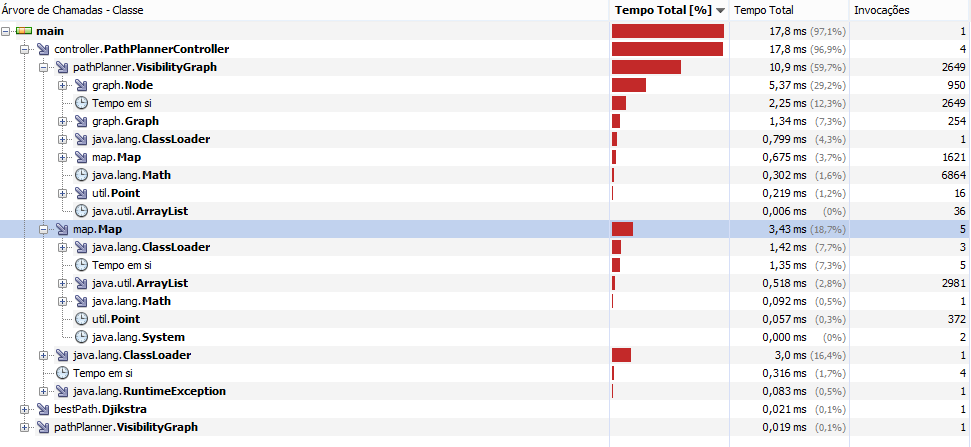
\includegraphics[keepaspectratio=true,scale=0.6]{figuras/visib3.PNG}
	\caption{tempo de processamento do mapa 3 com Grafo de Visibilidade}
\end{figure}

\begin{figure}[H]
	\centering
	\label{fig49}
		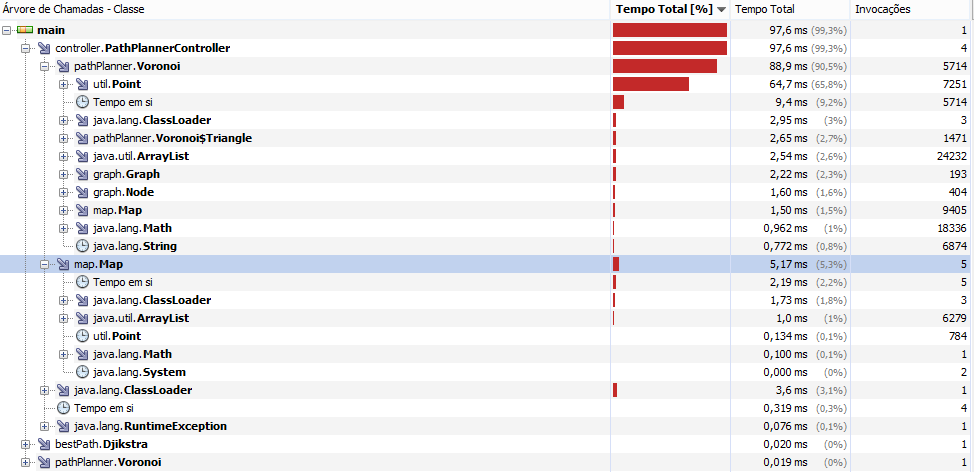
\includegraphics[keepaspectratio=true,scale=0.6]{figuras/voronoi3.PNG}
	\caption{tempo de processamento do mapa 3 com Voronoi}
\end{figure}

\begin{figure}[H]
	\centering
	\label{fig50}
		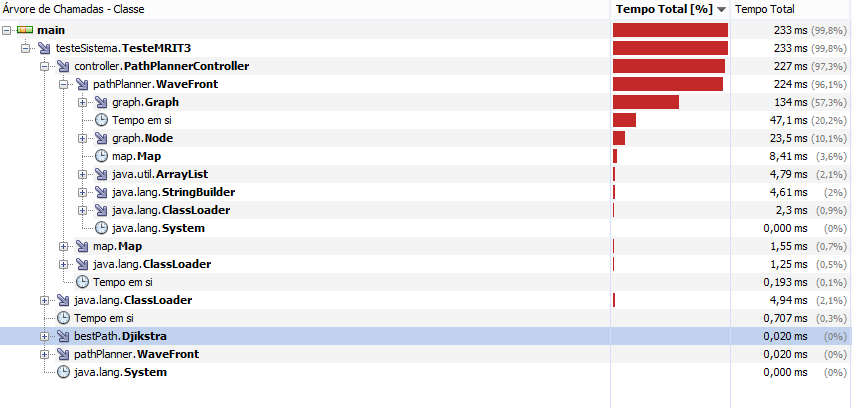
\includegraphics[keepaspectratio=true,scale=0.6]{figuras/wave3.PNG}
	\caption{tempo de processamento do mapa 3 com Wavefront}
\end{figure}

\section{Testes Finais Com o Robô}

Com o código-fonte do Traveller concluída e de posse dos resultados das simulações, foi realizado um teste final com o robô, verificando os quatro algoritmos. Foi inserido no robô o módulo EmbeddedCommunication e executado a classe concreta NXTCommunication. O mapa inserido na memória foi o mapa 1. Como servidor foi usado um notebook comum, rodando o código do Traveller e com o Bluecove inserido para a comunicação \textit{bluetooth}. 

O robô executou toda a comunicação de forma correta, enviando e recebendo os dados sem perdas nem alterações. O robô recebeu a lista de pontos e executou a movimentação entre os mesmos para os quatro algoritmos.

Por fim, foi medido o tempo da comunicação entre o robô e o servidor. Para tanto, foi utilizado a biblioteca do próprio Java implementado no robô. Foram medidos dois tempos: o tempo para abrir a comunicação entre o robô e o servidor e o tempo para enviar os dados, o Traveller executar todo o fluxo de trabalho e enviar a resposta de volta para o robô. Para cada algoritmo foi medido três veses estes dois valores.

A abertura da comunicação entre as partes, em todas as 12 medidas, levou entre 4.6 segundos e 7.8 segundos. A média de tempo foi de 5.5 segundos. Para os algoritmos, o tempo de processamento real foi de: i) Quadtree teve média de 4.981 ii) Wavefront teve média de 7.078 segundos iii) Grafo de Visibilidade teve média de 4.389 segundos e iv) Voronoi teve média de 4.393 segundos.

Os tempos reais foram bastante discrepantes com os valores simulados, porém uma proporção se manteve. Em ambos os casos, o algoritmo Wavefront levou muito mais tempo que os demais. Enquanto os outros três algoritmos levaram entre 4 e 5 segundos, o Wavefront levou, em todas as medições, pouco mais de 7 segundos. O Quadtree consumiu um pouco de tempo a mais que o Voronoi e o Grafo de Visibilidade, sendo o único dos três a passar de 5 segundos em alguma medida e ficando com uma média de mais de meio segundo acima dos outros dois. Não houve uma diferença considerável entre o Voronoi e o Grafo de Visibilidade. Os valores das medidas podem ser vistos na Tabela 7.

\begin{table}[h]
	\centering
	\label{tab07}
	\begin{tabular}{c|c|c|c}
		\toprule
		\textbf{Algoritmo} & \textbf{Medida 1} & \textbf{Medida 2} & \textbf{Medida 3} \\
		\midrule
Grafo de Visibilidade & 4,965s  & 5,022s & 4,956s \\
Voronoi 				  & 7,011s  & 7,216s & 7,008s \\
Quadtree				  & 4,462s  & 4,366s & 4,340s \\
Wavefront             & 4,393s  & 4,365s & 4,422s  \\
		\bottomrule
	\end{tabular}
	\caption{Tempos reais gasto pelos algortimos}
\end{table}

\section{Observações Sobre o Funcionamento dos Algoritmos}

Uma observação importante a se fazer é em relação ao mapa 6. Ele foi desenhado propositalmente para que nenhum algoritmo conseguisse gerar um percurso nele. O ponto inicial foi cercado por obstáculos que, após expandidos, deixariam um espaço menor que a largura do robô e, assim, impedindo a geraão da trajetória. No simulador MRIT, o Grafo de Visibilidade conseguiu gerar uma solução mesmo com a distância entre os obstáculos sendo de uma célula e o robô ocupando duas.

No caso do Traveller, tanto o Grafo de Visibilidade quanto o Wavefront geraram uma solução. Este mapa permite avaliar algumas características importantes sobre os quatro algoritmos.

O Quadtree e o Voronoi não são capazes de gerar uma solução em um ambiente como o do mapa 6 por trabalharem com divisão espacial. Ambos os algoritmos dividem o mapa em reigões e as interliga, o que os torna inviáveis em ambientes muito apertados. Em um cenário como o do mapa 6, os algoritmos não são capazes de criar uma região tão pequena e acabam por desconsiderar corredores estreitos.

Já os algoritmos Grafo de Visibilidade e Wavefront trabalham de forma linear. Ambos os algoritmos geram uma linha reta entre dois pontos quaisquer e, se essa linha reta for toda livre de obstáculos, então o robô poderá trafegar por ela.

No caso do Traveller, em específico, o Grafo de Visibilidade expande os obstáculos obrigatoriamente. Assim, mesmo que haja um corredor de apenas uma célula entre dois obstáculos expandidos, o algoritmo garantiu uma área de segurança de metade da largura de robô para cada lado. Desse modo, existe na verdade um percurso igual a largura do robô mais uma célula entre os obstáculos. O robô irá invadir a área de risco, porém não colidirá com os obstáculos e seu centro passará no centro entre os obstáculos.

Quanto ao Wavefront, este também considera que, se há ao menos uma célula livre entre os obstáculos expandidos, então há espaço suficiente para o robô se locomover entre eles. Porém, diferente do Grafo de Visibilidade, que força a expansão, o Wavefront não garante que essa expansão realmente ocorra. Se os obstáculos não forem expandidos e houver um percurso menor que a largura do robô, o algoritmo tentará passar por este corredor e a colisão ocorrerá.

\section{Resumo do Capítulo}

Os primeiros testes realizados visavam testar a capacidade  de memória do kit utilizado, criando mapas grande e com muitos obstáculos. Foi então dimunuídos esses valores gradativamente até que o robô fosse capaz de armazená-los. Com esses testes foi verificado que mesmo com um mapa não muito grande e com poucos obstáculos a memória não suportava esse volume de dados. Portanto, foi definido que o núcleo do sistema seria migrado para um servidor e comunicado com o robô via \textit{bluetooth}.

Foi realizado testes unitários e de integração do \textit{framework} desenvolvido, visando garantir a qualidade do código. Cada algoritmo desenvolvido tinha um conjunto de classes de teste que verificavam o correto funcionamento do mesmo. Métodos mais complexos da classe Map também foram testados diretamente por testes unitários.

Os testes de integração realizados envolveram seis ambientes diferentes, modelados e simulados no simulador MRIT. Foi medido o percurso para cada algoritmo em cada um dos seis mapas, tanto no simulador quanto no \textit{framework}. O Grafo de Visibilidade teve os mesmos resultados ou muito próximos, o Quadtree teve resultados um pouco maiores e menos retilíneos, o Wavefront teve resultados consideravelmente menores e o Voronoi conseguiu solucionar apenas um dos mapas.

Foram realzadas simulações do processamento do Traveller, visando mensurar seu tempo de processamento. Porém, quando comparado aos valores reais medidos ao implantá-lo no robô, foram bastante discrepantes e apenas uma das proporções foi mantida.